\par
L'application est structurée selon un modèle MVC (Modèle Vue Contrôleur). Les données sont représentées par les classes du modèle, sont traitées par les classes du contrôleur et affichées par la vue. Nous utilisons en outre le patron de conception\footnote{Un patron de conception (souvent appelé design pattern) est un arrangement caractéristique de modules, reconnu comme bonne pratique en réponse à un problème de conception d'un logiciel. Il décrit une solution standard, utilisable dans la conception de différents logiciels. (Wikipédia)} Façade, qui nous permet de limiter la dépendance de la vue au contrôleur à une seule classe. Nous schématisons ces interactions dans la figure suivante.

\begin{figure}[!h]
	\centering
   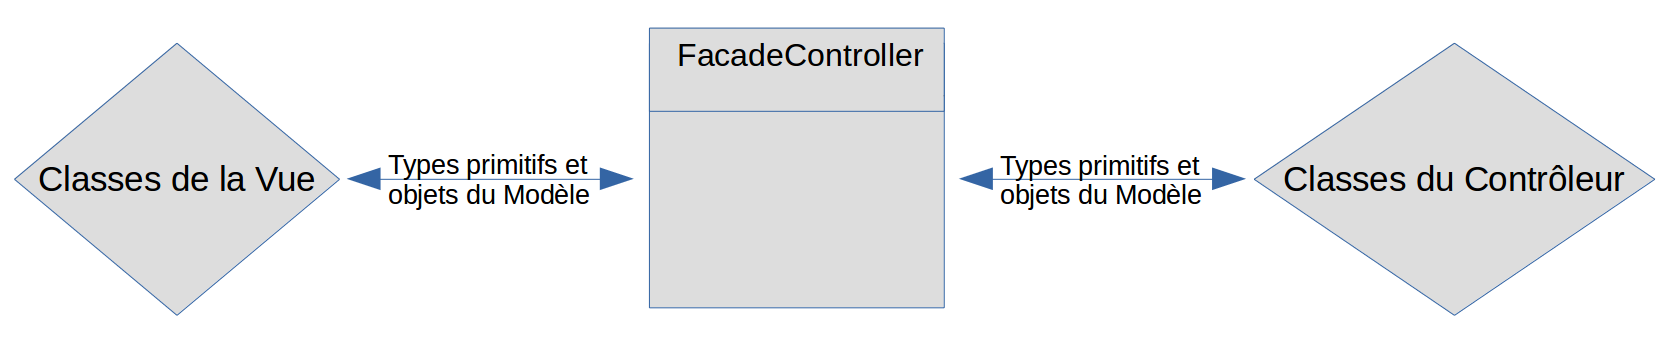
\includegraphics[scale=0.25]{img/facade.png}
   \caption{Interactions entre la vue et le contrôleur à travers la classe FacadeController}
\end{figure}

\par
Le modèle permet de représenter les QR Codes des différents types (voir \ref{typesQR}). Il est composé d'une superclasse abstraite \classe{QRCode}, étendue par deux classes \classe{QRCodeAtomique} et \classe{QRCodeEnsemble} représentant les spécificités des deux types de QR Codes gérés. Le modèle n'effectue pas de traitement des données mais fournit seulement des méthodes permettant d'y accéder et de les modifier, en faisant une abstraction de la façon dont elles sont représentées. Le diagramme UML des classes du modèle est visible ci-dessous.

\begin{figure}[!h]
	\centering
   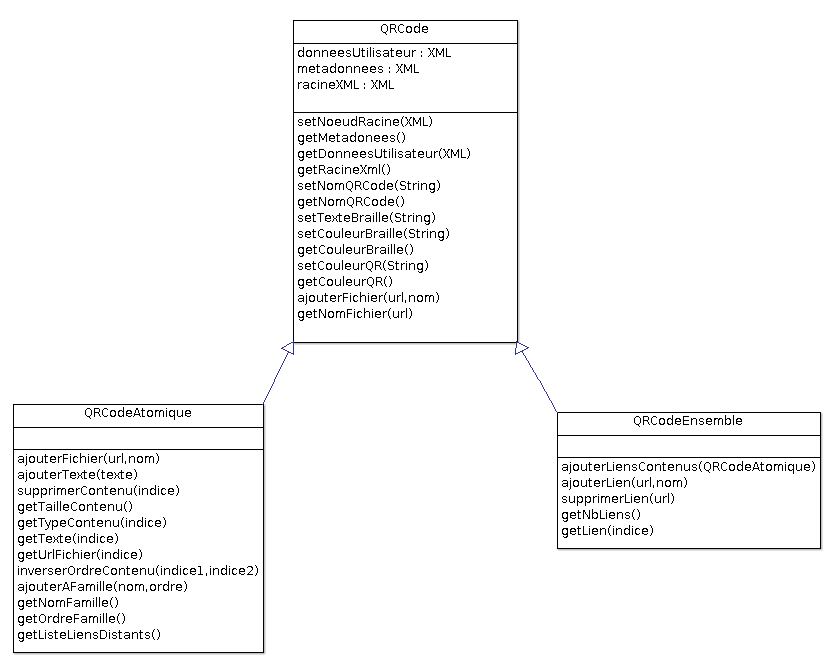
\includegraphics[scale=0.4]{img/modeleUML.png}
   \caption{Diagramme UML des classes du modèle}
\end{figure}

\par
Le contrôleur se charge de tous les traitements permettant de générer des images de QR Codes (voir \ref{generation}), ou d'instancier des objets du modèle à partir d'une image déjà générée (voir \ref{chargement}). L'architecture des classes du contrôleur est visible ci-dessous.


\begin{figure}[!h]
	\centering
   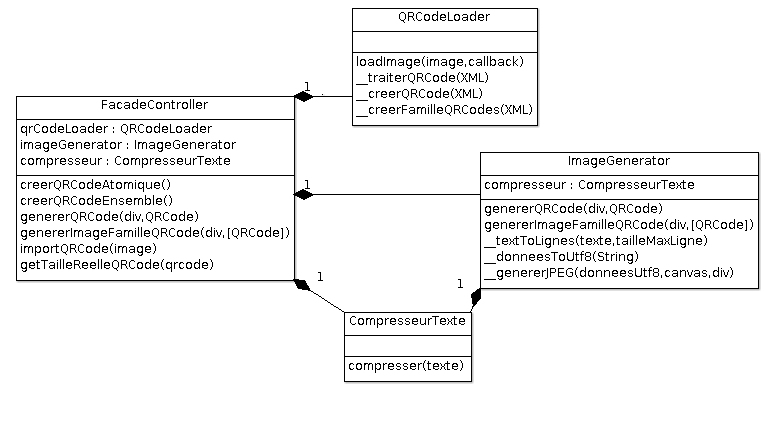
\includegraphics[scale=0.4]{img/controllerUML.png}
   \caption{Diagramme UML des classes du contrôleur}
\end{figure}

\par
La vue est elle responsable des interactions avec l'utilisateur (voir \ref{interfaceGraphique}). Elle offre une interface permettant de charger, de créer, d'afficher et de gérer des QR Codes.